%-------------------------------------------------------
\section{In the Beginning}
\subsection{The United States}
%-------------------------------------------------------
\begin{frame}{In the Beginning}{The United States}
%-------------------------------------------------------
	\begin{itemize}
		\item<1 -> Settled by Christians - the Puritans.
		\item<2 -> Founded on science - logic and reason.
			\begin{itemize}
				\item<3 -> Logic and reason helped ensure religious freedom
				\item<3 -> This is why religious mentality was not incorporated into the Declaration of Independence
			\end{itemize}
	\end{itemize}
\end{frame}

%-------------------------------------------------------
\subsection{God's Natural Law is Reason}
%-------------------------------------------------------
\begin{frame}{In the Beginning}{God's Natural Law is Reason}
%-------------------------------------------------------
	\begin{columns}[c]
		\column{0.6\textwidth}
			From approx. 700 C.E. to 900 C.E.\\
			\begin{itemize}
				\item Mu'tazilites mode of study
					\begin{itemize}
						\item Discern God's will by studying nature
						\item God speaks through nature
					\end{itemize}
			\end{itemize}
		\column{0.4\textwidth}
			\begin{figure}
				\centering
				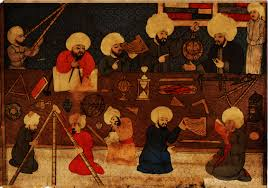
\includegraphics[width=\textwidth]{images/mutazilite_science}
				\caption{Mu'tazilite Science}
			\end{figure}
	\end{columns}
\end{frame}

%-------------------------------------------------------
\begin{frame}{In the Beginning}{God's Natural Law is Reason}
%-------------------------------------------------------
	\begin{columns}[c]
		\column{0.6\textwidth}
			1517 C.E.
			\begin{itemize}
				\item Martin Luther nails his 95 theses to the door of a Catholic church to protest the Church's practices
					\begin{itemize}
						\item Protestants argued that knowledge comes from observing God's Word, not the Pope's word
					\end{itemize}
			\end{itemize}
		\column{0.4\textwidth}
			\begin{figure}
				\centering
				
\includegraphics[width=\textwidth]{images/martin_luther}
				\caption{Martin Luther}
			\end{figure}
	\end{columns}
\end{frame}

%-------------------------------------------------------
\begin{frame}{In the Beginning}{God's Natural Law is Reason}
%-------------------------------------------------------
	\begin{columns}[c]
		\column{0.6\textwidth}
			1518 C.E.
			\begin{itemize}
				\item Protestant polemicist St. Germain supports "do it yourself" Bible study
					\begin{itemize}
						\item Protestants argued that knowledge comes from observing God's Word, not the Pope's word
						\item Use one's own experience of the Bible to find truth\\
							This approach is in the same "anti-authoritarian" vein as the modern scientific approach (make observations, then come to conclusions)
					\end{itemize}
			\end{itemize}
		\column{0.4\textwidth}
			\begin{figure}
				\centering
				
\includegraphics[width=\textwidth]{images/martin_luther}
				\caption{Martin Luther}
			\end{figure}
	\end{columns}
\end{frame}

%-------------------------------------------------------
\begin{frame}{In the Beginning}{God's Natural Law is Reason}
%-------------------------------------------------------
	\begin{columns}[c]
		\column{0.6\textwidth}
			Early 1600's
			\begin{itemize}
				\item Puritan sympathizer Edward Coke argues that scientific laws could be studied by everyone, and could not be overruled by the crown.
			\end{itemize}
		\column{0.4\textwidth}
			\begin{figure}
				\centering
				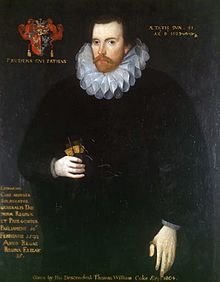
\includegraphics[width=\textwidth]{images/edward_coke}
				\caption{Edward Coke}
			\end{figure}
	\end{columns}
\end{frame}

%-------------------------------------------------------
\begin{frame}{In the Beginning}{God's Natural Law is Reason}
%-------------------------------------------------------
	\begin{columns}[c]
		\column{0.6\textwidth}
			Late 1500's to mid 1600's
			\begin{itemize}
				\item Puritans supported a logical, antiauthoritarian approach to theology:
					\begin{itemize}
						\item Making your own observations from the Bible and not relying on the Pope
						\item Use observations to draw broader theological conclusions
						\item Puritans study Mu'tazilite science books
					\end{itemize}
			\end{itemize}
		\column{0.4\textwidth}
			\begin{figure}
				\centering
				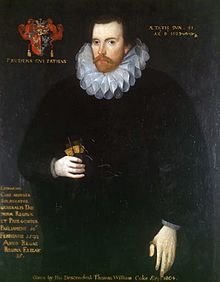
\includegraphics[width=\textwidth]{images/edward_coke.png}
				\caption{Edward Coke}
			\end{figure}
	\end{columns}
\end{frame}



% Timeline of Events:

% ~A.D. 700-900: Mu’tazilites mode of study: Discern God’s will by studying nature
% God speaks through nature
% 1517: Beginning of the Protestant Reformation 
% Martin Luther nails his 95 Theses, in protest of the Catholic Church’s practices
% Protestants argued that knowledge comes from observing God’s Word, not the Pope’s word
% 1518: Protestant polemicist St. Germain supports “do it yourself” Bible study
%           - Use one own’s experience of the Bible to find truth
%           - This approach used was of the same “antiauthoritarian” nature of the emerging (now modern) scientific approach (make observations, then come to conclusion)

% Early 1600s: Puritan sympathizer Edward Coke argues that scientific laws could be studied by everyone, and could not be overruled by the crown.

% Late 1500s to mid-1600s:  Puritans supported a logical, antiauthoritarian approach to theology:
% Making your own observations from the Bible and not relying on the Pope
% Use observations to draw broader theological conclusions
% Puritans study Mu’tazilite science books
